\documentclass[main, 12pt, fleqn]{subfiles}

\begin{document}

\begin{lect} {2019-10-09}
	\begin{proof}
	    Продолжение
		\[\text{п3 } f^{-1} \text{ - непр. диф? } \rla \]
		\[g = f^{-1} : V \to U_a \qq d_g : V \to \L (\R^n, \R^{2n} ) \]
		\[d_g \in C(V)\]
		\[\forall y \in V \q y \us{\text{непр?}}{\to } d_{y} g \]
		\[(\text{п. 4}) \q d_y g = \left(d_{g(y)} f \right)^{-1} \qq f \circ g = id \qq (f \circ g)(y) = y\]
		\[d_{g(y)} f \cdot d_y g = E_n\]
		\[y \to d_y g\]
		\[y \to g(y) \to d_{g(y)} f \to (d_{g(y)} f )^{-1}  \]
		\[\text{т.е } y \to d_y g \text{ - композиция трех непр. отображений}\]
	\end{proof}

	\begin{Example}
		\[f(\rho, \varphi) = \begin{pmatrix}
			\rho \cos \varphi\\
			\rho \sin \varphi
		\end{pmatrix} \begin{align}
				\leftarrow f_x\\
				\leftarrow f_y
		\end{align}\]
		\[f : (0; + \infty) \times \R \to \R^2\]
		\[\det(d_{\rho, \varphi} f ) = \det \begin{pmatrix}
			\frac{\partial f_x}{\partial \varphi} & \frac{\partial f_x}{\partial \varphi}\\
			\frac{\partial f_y}{\partial \varphi} & \frac{\partial f_y}{\partial \varphi}
		\end{pmatrix} =
		\det \begin{pmatrix}
			\cos \varphi & - \rho \sin \varphi\\
			\sin \varphi & \rho \cos \varphi
		\end{pmatrix} = \rho \neq 0 \]
		\[\Ra \text{ по теор. об обратном отобр } \exists \text{ лок. отобр}\]
		\[\text{Но } \not \exists \text{ глобального обр. отобр. (т.к. не биекция)}\]
	\end{Example}

	\begin{Consequence} [об открытом отображении]
		\[\letus\ U \subset \R^n \text{ - откр.} \q f \in C^{1}(U)\]
		\[\forall a \in U \q d_{a} f \text{ - обратим} \]
		\[\text{Тогда } \forall E \subset U \q E \text{ - откр. } \q f(E) \text{ - откр.}\]
	\end{Consequence}

	\begin{Proof}
		\[\letus\ b \in f(E) \Ra \exists a \in \us{\text{откр}}{E} : f(a) = b \text{ (пробраз)}\]
		\[\Ra \exists \us{}{ U_a} \ni a \q U_a \subset E : \]
		\[f : U_a \to \us{\text{откр из теор об обр отобр}}{f(U_a)} \text{ - биекция}\]
		\[b \in f(U_a) \subset f(E)\]
	\end{Proof}

	\subsection{Теорема о неявном отображении}

	\begin{Examples}
		%рисунок 1
		\begin{figure}[H]
		    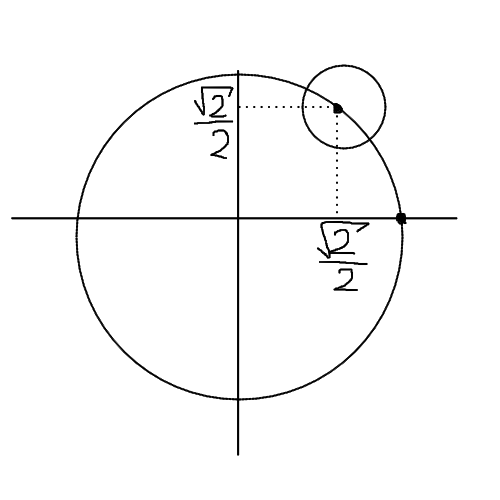
\includegraphics[scale=2]{pics/6_1.png}
		    \centering
		\end{figure}

		\[1)\]
			\[ x ^ 2 + y^2 = 1\]
			\[y(x) - ?\]
			\[M_1 (\frac{\sqrt{2}}{2}, \frac{\sqrt{2}}{2}) \q \text{ в окр. } M_1 \q x^2 + y^2 = 1 \q
			y = \sqrt{1 - x^2} \q x \in (0, 1)\]
			\[M_2 \left(\frac{\sqrt{2}}{2}, -\frac{\sqrt{2}}{2}\right) \text{ в окр. } M_2 \q
			y = - \sqrt{1 - x^2}\]
			\[M_3(1, 0 ) \text{ - не получается}\]
			\[\Phi(x, y) = x^2 + y^2 - 1\]
			\[\Phi'_y = 2y\]
		\[2)\]
			\[\begin{cases}
					y_1 + y_2 = x_1\\
					y_1 - y_2 = x_2
			\end{cases}\]
			\[\Phi(x_1, x_2, y_1, y_2) = \begin{pmatrix}
				y_1 + y_2 - x_1\\
				y_1 - y_2 - x_2
			\end{pmatrix} =
		\begin{pmatrix}
			0\\
			0
		\end{pmatrix}\]

		\[y_1(x_1,x_2); \ y_2(x_1, x_2)\]
		\[y_1 = \frac{x_1 + x_2}{2} \ y_2 = \frac{x_1 - x_2}{2}\]
		\[\begin{cases}
			ay_1 + by_2 = x_1\\
			cy_1 + dy_2 = x_2
		\end{cases} \text{ - однозн. разрешима от } y_1 \text{ и } y_2 \rla \begin{vmatrix}
		a & b\\
		c & d
	\end{vmatrix} \neq 0\]

	Обозначения
	\[\Phi: \us{(x, y)}{W} \subset \R^{n + m} \to \R^{m}  \]
	\[\R = \us{x}{\R^n} \times \us{y}{\R^m}\]
	\[\det(d_{(x_y)} \Phi ) = \begin{pmatrix}
		\frac{\partial \Phi_1}{\partial x_1} & ... & \frac{\partial \Phi_1}{\partial x_n} &
		\frac{\partial \Phi_1}{\partial y_1} & ... & \frac{\partial \Phi_1}{\partial y_m}\\
		...\\
		\frac{\partial \Phi_m}{\partial x_1} & ... & \frac{\partial \Phi_m}{\partial x_n} &
		\frac{\partial \Phi_m}{\partial y_1} & ... & \frac{\partial \Phi_m}{\partial y_m}

	\end{pmatrix} (x, y)\]
	\[\Phi(x_1, x_2, y_1, y_2) = \begin{pmatrix}
		ay_1 + by_2 - x_1\\
		cy_1 + dy_2 - x_2
	\end{pmatrix} = 0 \qq \Phi_y' = \begin{vmatrix}
	a & b\\
	c & d
	\end{vmatrix} \neq 0\]
	\end{Examples}

	\begin{Theorem} [О неявном отображении]
		%рисунок 2
		\begin{figure}[H]
		    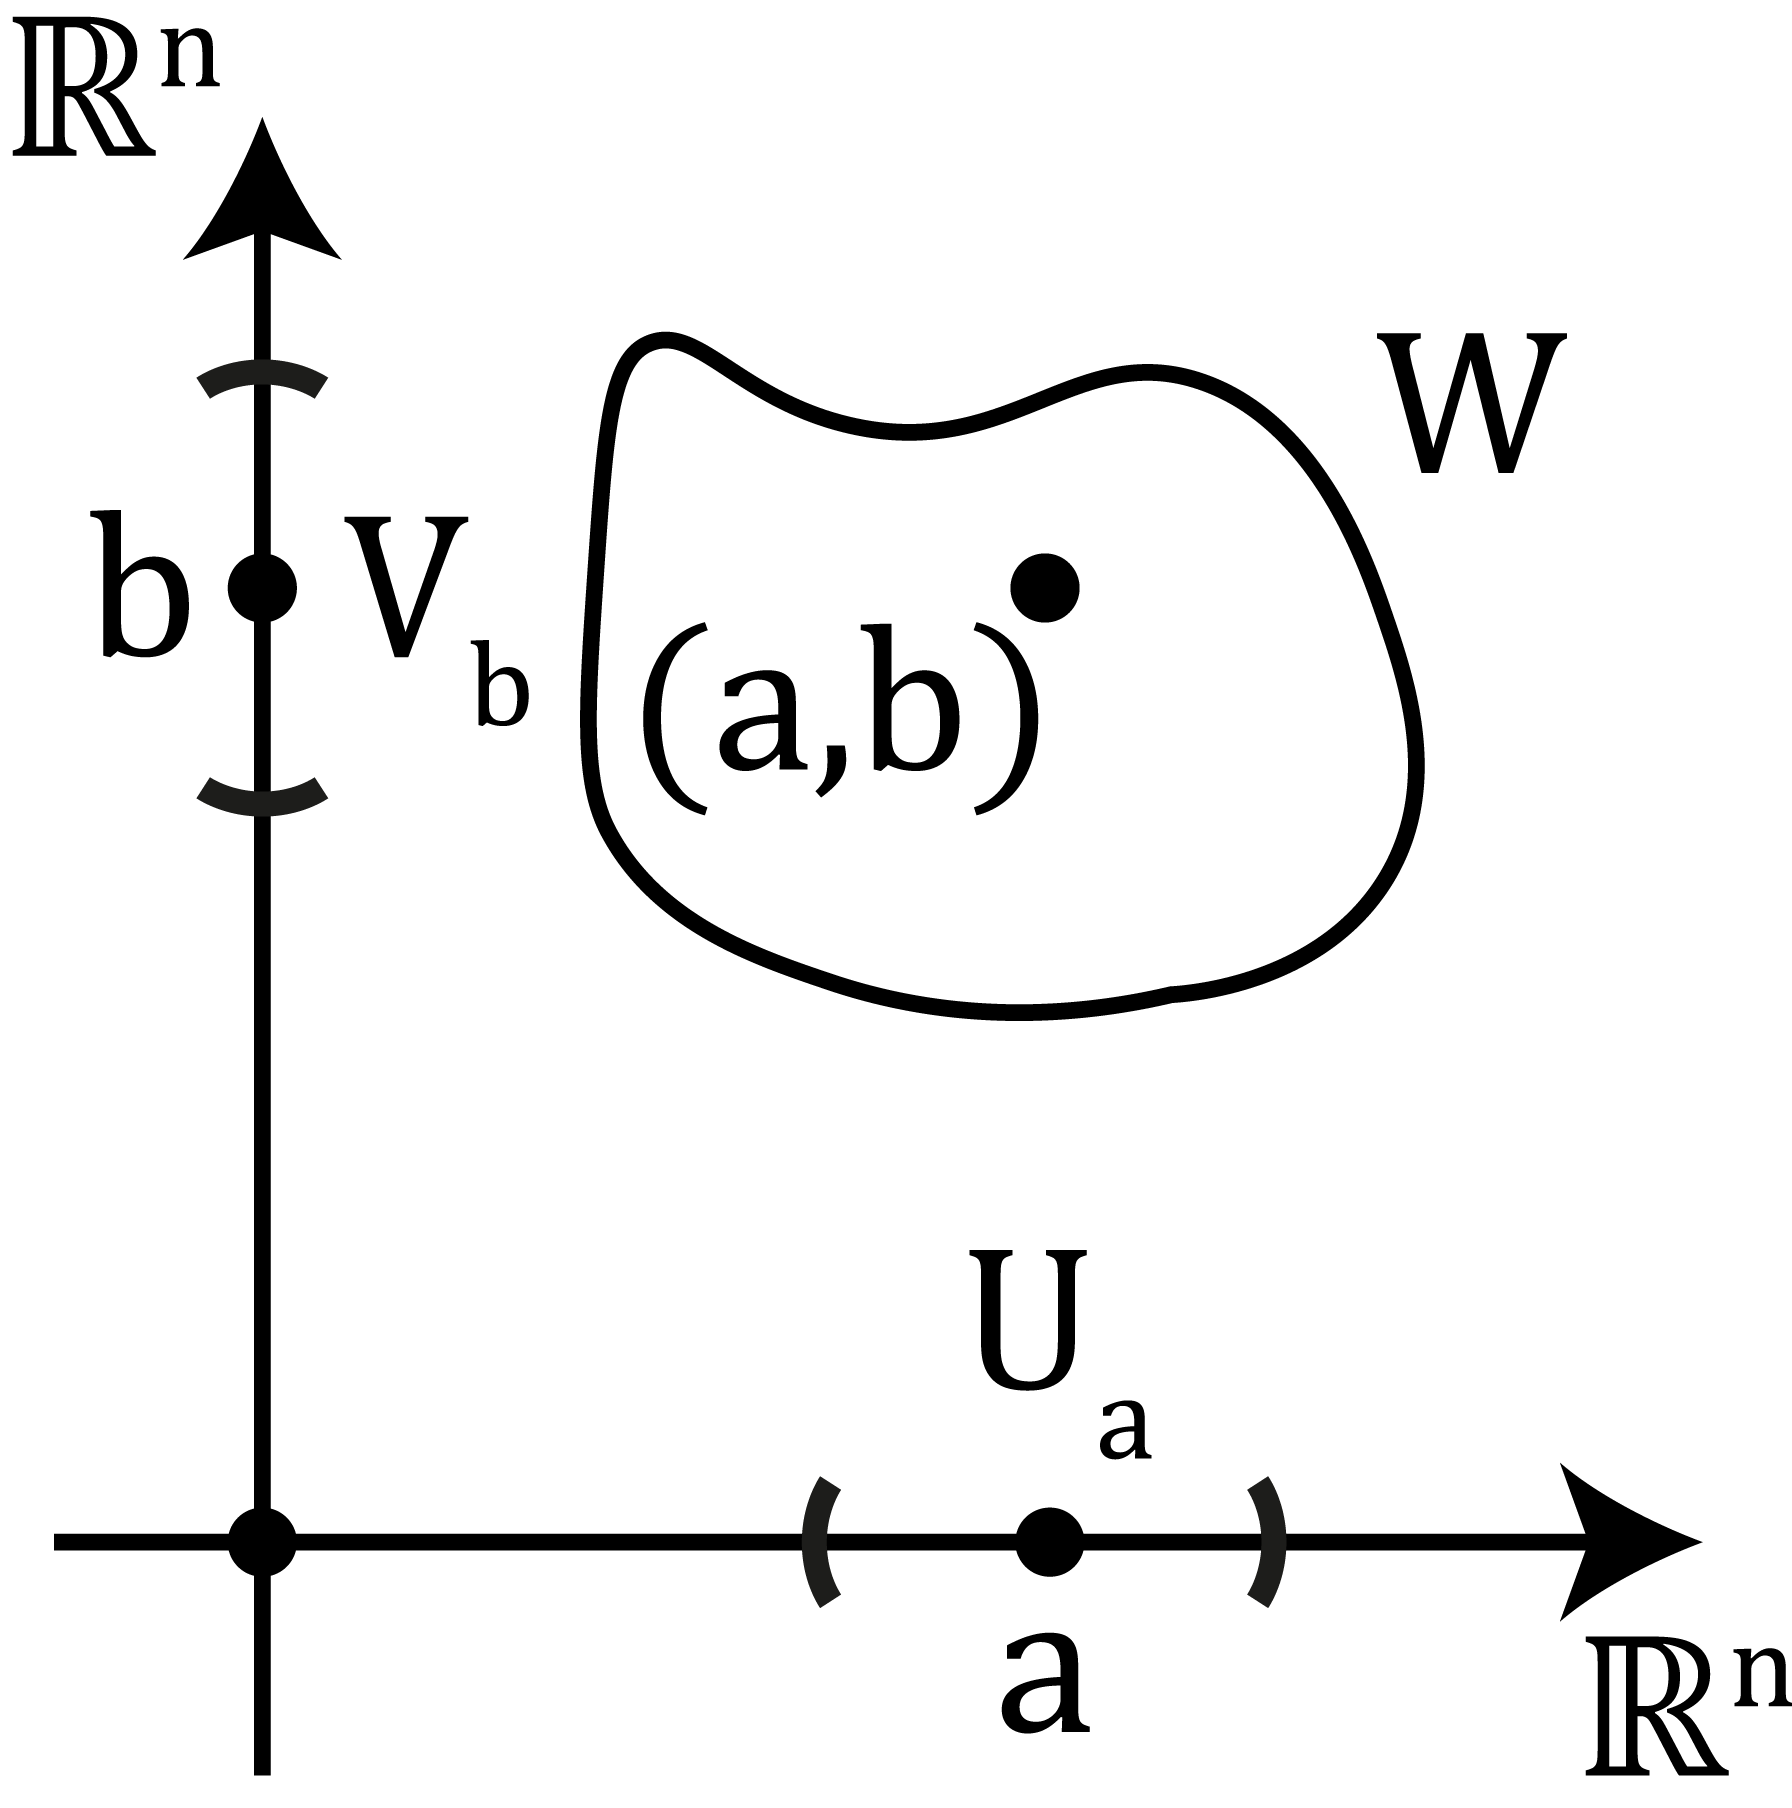
\includegraphics[scale=2]{pics/6_2}
		    \centering
		\end{figure}

		\[\us{\text{откр}}{W} \subset \R^{n + m}  \qq (a, b) \in W\]
		\[\Phi : W \to \R^m \q \Phi \in C^{1} (W) \q W(a, b) = 0_m \in \R^m\]
		\[\det(\Phi'_y(a, b)) \neq 0 \q \text{Тогда}\]
		\[\exists U_a \text{ - окр. } a \q V_b \text{ - окр. }b\]
		\[1) \q \forall x \in U \q \exists ! y \in V : \Phi (x, y) = 0\]
		\[(\text{Обозначим } \varphi(x) = y (\text{который ед}))\]
		\[\text{т.е } \exists \text{ отобр } \varphi : U \to V :  \q \Phi(x, \varphi(x)) = 0\]
		\[2) \q \varphi \in C^{1}(U \to V)\]
		\[3) \q \varphi'(x) = - \left(\Phi_y'(x, y)\right)^{-1} \left(\Phi'_x(x, y)\right)
		\bigg|_{y = \varphi(x)} = \]
		\[= - (\Phi_y'(x, \varphi(x)))^{-1}(\Phi_x'(x, \varphi(x)))  \q \forall x \in U\]
		\[\Phi(x, \varphi(x)) = 0\]
		\[\frac{\partial \Phi}{\partial x} + \frac{\partial \Phi}{\partial y} \cdot \varphi'(x) = 0\]
		\[\varphi'(x) = - \frac{\Phi_x'(x, y)}{\Phi'_y(x, y)}\]
	\end{Theorem}


	\begin{Proof}
		\[F(x, y) = (\us{\in \R^n}{x}, \us{\in \R^m}{\Phi(x,y)}) \in \R^{n + m}\]
		\[F \begin{pmatrix}
			x_1\\
			\vdots\\
			x_n\\
			y_1\\
			\vdots\\
			y_m
		\end{pmatrix} =
		\begin{pmatrix}
			x_1\\
			\vdots\\
			x_n\\
			\Phi_1(x,y)\\
			\vdots\\
			\Phi_m(x, y)
		\end{pmatrix}
		\q F : W \to \R^{n + m} \]
		\[F \in C^{1}(W) \]
		\[\Phi'_y(a, b) - \text{ обратим}\]
		\[F'(a, b) = d_{(a, b)} F =
		\begin{pmatrix}
			1 & 0 & 0  & ... & 0\\
			0 & 1 & 0  & ... & 0\\
			...\\
			0 & .. &  1 & ... & 0\\
			\frac{\partial \Phi_1}{\partial x_1} & ... & \frac{\partial \Phi_1}{\partial x_n} &
			\frac{\partial \Phi_1}{\partial y_1} & ... & \frac{\partial \Phi_1}{\partial y_m}\\
			...\\
			\frac{\partial \Phi_m}{\partial x_1} & ... & \frac{\partial \Phi_m}{\partial x_m} &
			\frac{\partial \Phi_m}{\partial y_1} & ... & \frac{\partial \Phi_m}{\partial y_m}

		\end{pmatrix} \Bigg|_{(a, b)} = \]
		\[= \begin{pmatrix}
			E_n & 0_{n \times m}\\
			\Phi'_x(a, b) & \Phi_y'(a, b)
		\end{pmatrix}\]
		\[\det F'(a, b) = \det \Phi'_y(a, b) \neq 0\]
		\[\text{т.е. } F'(a, b) \text{ - обратим} \]
		\[\text{Применим теор. об обратном отобр. к } F\]
		\[\exists\ W_0 \text{ - окр. т. } (a, b) : F(W_0) \text{ - откр.}\]
		\[F : W_0 \to F(W_0) \text{ - биекция и }F'(x, y) \text{ - обратим } \forall (x, y) \in W_0\]
		\[F(a, b) = (a, 0)\]
		\[\letus U_a \text{ - окр. } a\]
		\[V_b \text{ - окр. } b:\]
		%рисунок 3
		\begin{figure}[H]
		    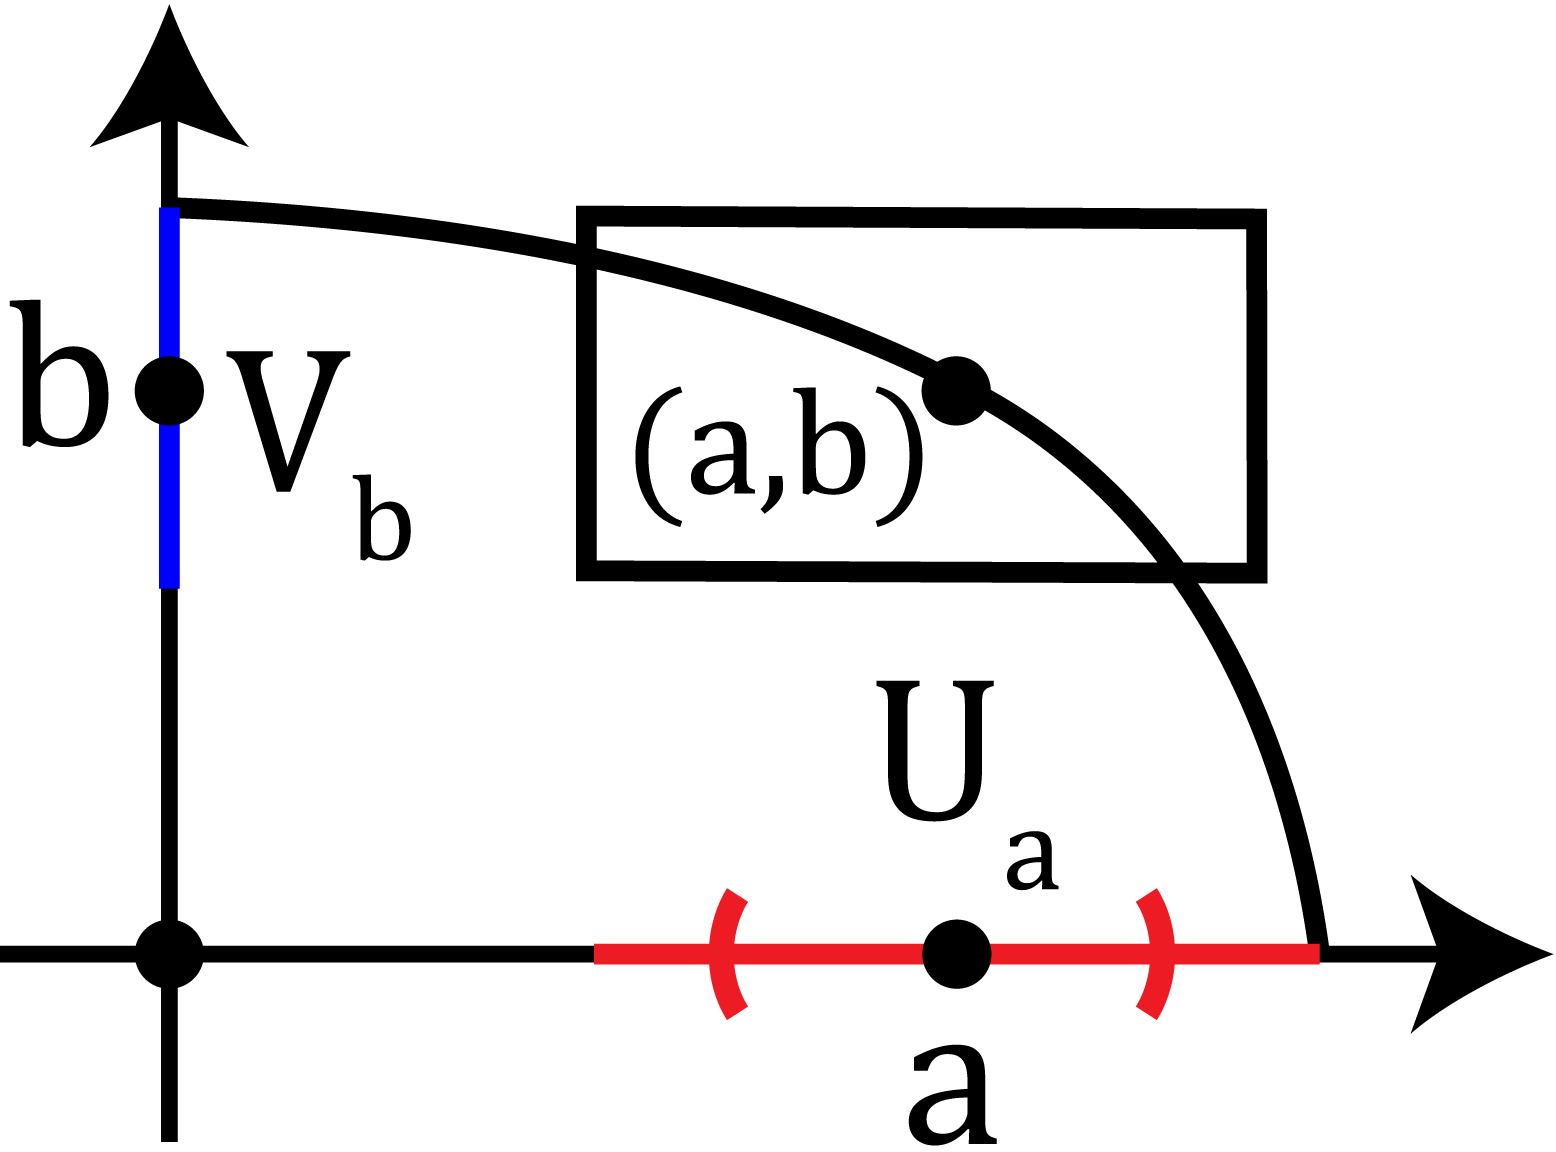
\includegraphics[scale=2]{pics/6_3}
		    \centering
		\end{figure}

		\[\os{\text{откр}}{U_a \times V_b} \subset W_0\]
		\[\text{по след-ю об открытом графике}\]
		\[F(U_a \times V_b) \text{ - откр.}\]
		\[\exists\ U \text{ - окр } a : \forall x \in U \Ra (x, 0) \in F(U_a \times V_b)\]
		\[\text{Покажем, что}\]
		\[U, V = V_b \text{ - то, что надо}\]
		\[\forall x \in U \Ra \us{\exists y \in V_b : = F(x, y)}{(x, 0)} \in F(U \times V_b)\]
		\[\text{Почему ед } y?\]
		\[\letus\ \exists \widetilde{y} \in V_b : F(x, \widetilde{y}) = (x, 0)\]
		\[\us{\in U \times V_b}{F(x, y)} = \us{\in U \times V_b}{F(x, \widetilde{y})} = (x, 0)\]
		\[\text{т.к. } F \text{ - обр на } U \times V_b \Ra y = \widetilde{y}\]
		\[\Ra \exists \text{ обр отобр}\]
		\[F^{-1}(x,0) = (x, y) \]
		\[F(x, 0) = F(x, y) = (x, \Phi(x, y))\]
		\[\Phi(x, y) = 0\]
		\[\text{т.о } \forall x \in U \q \exists !y = \varphi(x) : \q \Phi(x, \varphi(x)) = 0\]

		\[x \in \R^n \to (x, 0_m) \in \R^{n = m} \us{F^{-1} }{\to} (x, y) \to y \in \R^m  \text{ - это все }
		\varphi\]
		\[x \in \R^n\]
		\[Q : \R^n \to \R^{n + m} \]
		\[\Q(x) = (x, 0)\]
		\[\begin{pmatrix}
			E_n\\
			0_{m \times n}
		\end{pmatrix}
			\begin{pmatrix}
			x_1\\
			\vdots\\
			x_n
		\end{pmatrix} =
	\begin{pmatrix}
		x_1\\
		\vdots\\
		x_n\\
		0\\
		\vdots\\
		0
	\end{pmatrix} \qq \Q \in C^{\infty}(\R^n) \]
	    \[(x, y) \in \R^{n + m} \]
		\[P(x, y) = y \in \R^m \q (O_{n \times m} E_m )
		\begin{pmatrix}
			x_1\\
			\vdots\\
			x_m\\
			y_1\\
			\vdots\\
			y_m
		\end{pmatrix} =
	    \begin{pmatrix}
	    	y_1\\
			\vdots\\
			y_m
	    \end{pmatrix}
	\q P \in C^{\infty}(\R^n)\]
	\end{Proof}

	\begin{Proof}
		\[\text{п.3 } \q \Phi(x, \varphi(y)) = 0\]
		\[d_{(x, \varphi(x))} \Phi \cdot d_x (x, \varphi(x)) = 0_m\]
		\[d \begin{pmatrix}
			x\\
			\varphi(x)
		\end{pmatrix} =
	    \begin{pmatrix}
	    	E\\
			\varphi'(x)
	    \end{pmatrix} =
		\begin{pmatrix}
			1 & 0 & 0 & ... & 0\\
			...\\
			0 & 0 &   & ... & 1\\
			\frac{\partial \varphi_1}{\partial x_1} & & & & \frac{\partial \varphi_1}{\partial x_n}\\
			...\\
			\frac{\partial \varphi_m}{\partial x_1} & & & & \frac{\partial \varphi_m}{\partial x_n}
		\end{pmatrix}
	\]
		\[\begin{pmatrix}
			\frac{\partial \Phi_1}{\partial x_1} & ... & \frac{\partial \Phi_1}{\partial x_n} &
			\frac{\partial \Phi_1}{\partial y_1} & ... & \frac{\partial \Phi_1}{\partial y_n}\\
			...\\
			\frac{\partial \Phi_m}{\partial x_1} & ... & \frac{\partial \Phi_m}{\partial x_n} &
			\frac{\partial \Phi_m}{\partial y_1} & ... & \frac{\partial \Phi_m}{\partial y_m}
		\end{pmatrix}
		\Bigg|_{y = \varphi(x)}
		\begin{pmatrix}
			1 & 0 & 0 & ... & 0\\
			0 & 1 & ...\
			...\\
			0 & & & & 1\\
			\frac{\partial \varphi_1}{\partial x_1} & & & & \frac{\partial \varphi_1}{\partial x_n}\\
			...\\
			\frac{\partial \varphi_m}{\partial x_1} & & & & \frac{\partial \varphi_m}{\partial x_n}
		\end{pmatrix}\]
		\[(\Phi_x'(x, y) | \Phi'_y(x, y)) \begin{pmatrix}
			E\\
			\varphi'(x)
		\end{pmatrix} = 0\]
		\[\Phi'_x(x, y) + \Phi'_y(x, y) \cdot \varphi'(x) \bigg|_{y = \varphi(x)}  = 0\]
		\[\varphi'(x) = - (\Phi_y(x,y))^{-1} \cdot \Phi'_x(x, y) \bigg|_{y = \varphi(x)}  =
		-(\Phi_y'(x, \varphi(x)))^{-1}  \cdot \Phi_x'(x, \varphi(x))\]
	\end{Proof}

	\subsection{Условный экстремум}
	\begin{Definition}
		\[f : \us{\text{откр}}{W} \subset \R^{m + n} \to \R^1 \]
		\[\Phi : W \to \R^{m} \]
		\[x^0 \in W\]
		Если $\Phi(x^0) = 0$ и $\exists\ U_0 $ - окр-ть $x^0:$
		\[\forall x \in U_0 \cap W : \Phi(x) = 0 \Ra f(x^0) \geq f(x)\]
		\[\text{Тогда говорят, что } x^0 \text{ - точка условного } \max f \text{ при условии } \Phi(x) = 0\]
	\end{Definition}

	\begin{Example}
		\[f(x, y) = x^2 + y ^ 2\]
		\[\Phi(x, y) = x + y - 1\]
		\[\Phi(x, y) = 0 \rla x + y  = 1\]
		%рисунок 4
		\begin{figure}[H]
		    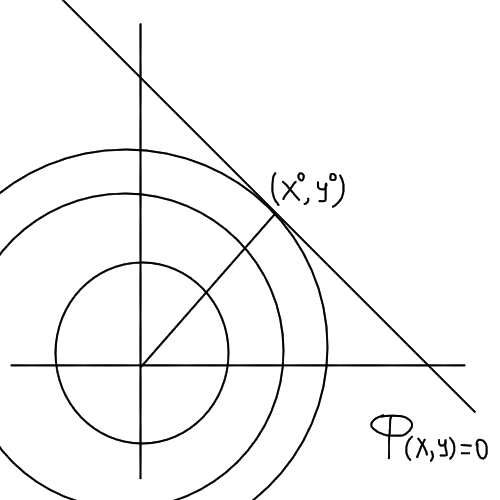
\includegraphics[scale=2]{pics/6_4}
		    \centering
		\end{figure}

		\[(x^0, y^0) \text{ - точка усл. } \min \Phi  f(x, y) \text{ при усл } \Phi(x, y) = 0\]
		\[\Phi(x, y) = Ax + By - c = 0\]
		\[f(x, y) = x^2 + y^2\]
		%рисунок 5

		\begin{figure}[H]
		    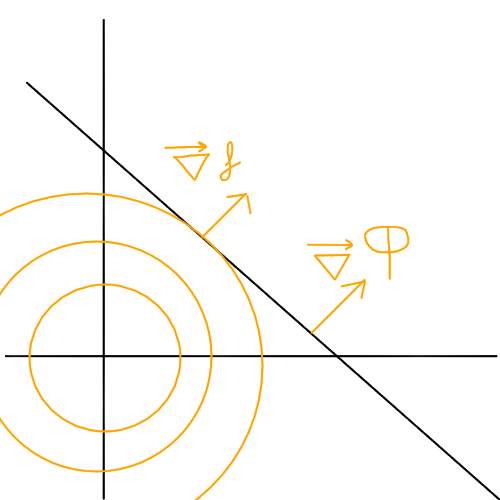
\includegraphics[scale=2]{pics/6_5}
		    \centering
		\end{figure}

		\[\Phi \in C^1(W \to \R^m) \text{ - m ур-ей (условия)}\]
		\[\begin{cases}
			\Phi_1(x_1, ..., x_{m+n}) & = 0\\
			\Phi_2(...) &= 0\\
			...\\
			\Phi_m(x_1, ..., x_{n + m}) &= 0
		\end{cases} \text{ - условия}\]
		\[f(x_1, ..., x_{n + m} ) \to \max (\min)\]
		Потребуем
		\[\rk \Phi'(x^0) = m \qq m \text{ - ЛНЗ столбцов}\]
		Перенумеруем $x_1, ..., x_{m + n} $ так, чтобы в $\Phi'(x^0)$ ЛНЗ последние $m$ столбцов\\
		%рисунок 6
		\begin{figure}[H]
		    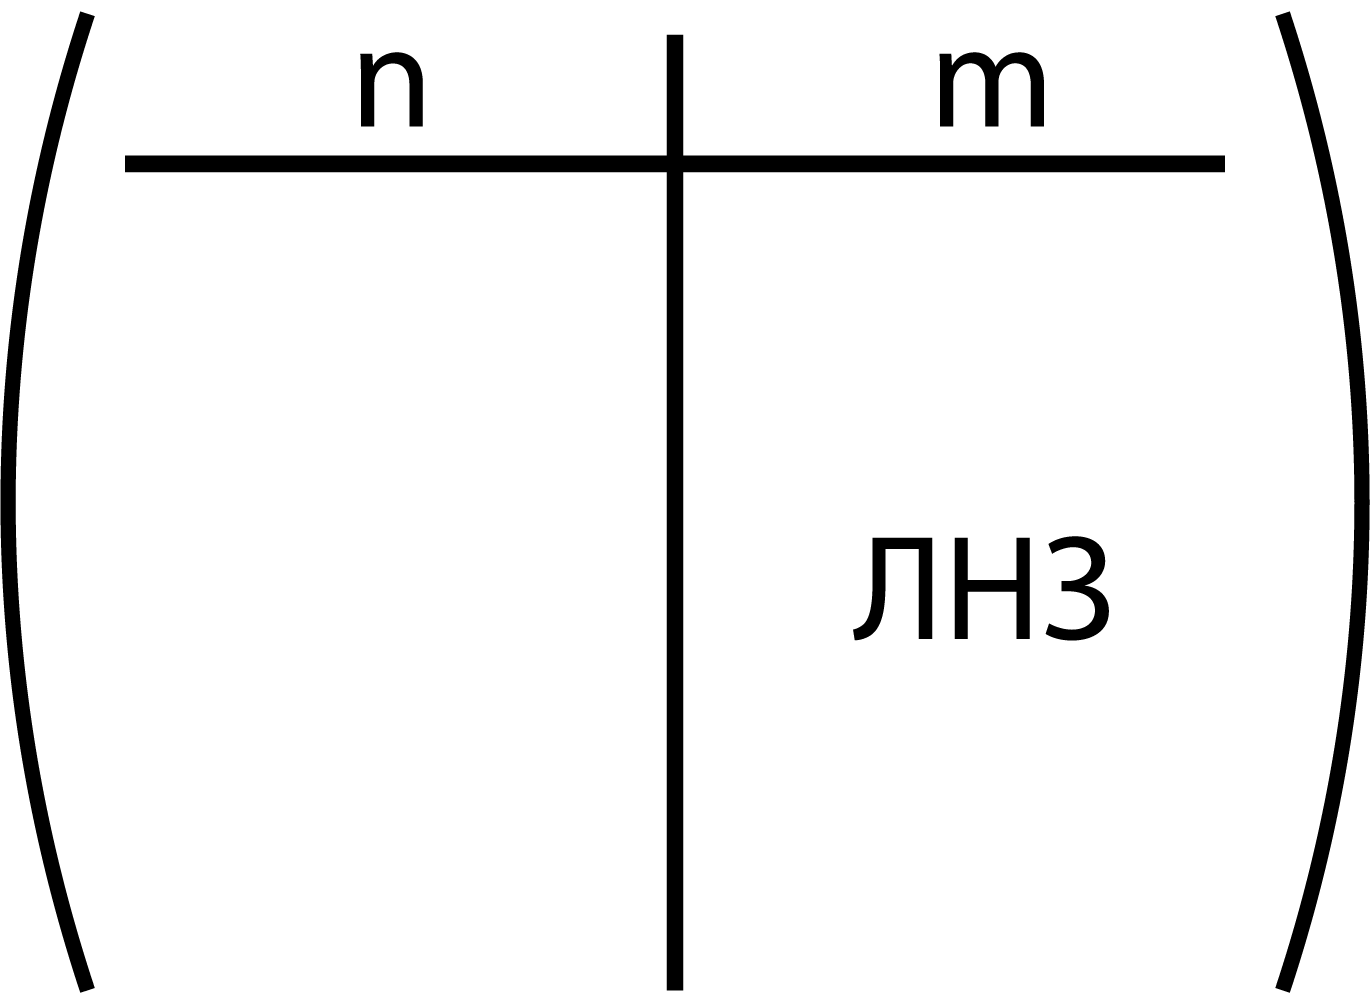
\includegraphics[scale=2]{pics/6_6}
		    \centering
		\end{figure}

		Переобозначим
		\[x_{n + 1} = y_1 \]
		\[x_{n + 1} = y_2\]
		\[...\]
		\[x_{n + m} = y_m\]
		\[\Phi(x_1, ..., x_n, y_1, ..., y_m) = 0_m \text{ - условие}\]
		\[\text{Причем } \Phi_y'(x^0) \text{ - обратим}\]
		\[x^0 = (a^0, b^0)\]
		\[\Phi(a^0, b^0) = 0\]
		\[\det(\Phi'_y(a^0, b^0)) \neq 0 \Ra \text{ по т. о неявной функции}\]
		\[\exists u, v, \q \varphi : u \to v : \q \Phi(x, \varphi(x)) = 0 \qq \varphi \in C^1(U)\]
		\[g(x) = f(\us{\in \R^n}{x}, \us{\in \R^{n + m} }{\varphi(x)}) \qq g : U \subset \R^n \to \R^1\]
		\[x^0 = (a^0, b^0) \qq b^0 = \varphi(a^0)\]
		\[\text{Если } x^0 \text{ - усл. } \max f \text{ при условии } \Phi(x) = 0 \text{, то}\]
		\[a^0 - \max \text{ функции } g(x) \Ra \]
		\[g'(a_0) = \nabla_{a^0} g = d_{a^0} g = 0 \]
		\[g(x) = f(x, \varphi(x))\]
		\[0 = g'(a^0) = f'_x (a^0, \varphi(a^0)) + f'_y (a^0, \varphi(a^0)) \cdot \varphi'(a^0) = 0\]
		\[(A) \qq f'_x (a^0, b^0) + f'_y (a^0, b^0) \varphi'(a^0) = 0\]
		\[\text{Продиф } \Phi(x, \varphi(x)) = 0\]
		\[(B) \qq \Phi'_x(a^0, b^0) + \Phi'_y(a^0, b^0) \cdot \varphi'(a^0) = 0_m\]
		\[\lambda = (\lambda_1, ..., \lambda_m) \in \R^m \text{ - множители Лангранжа}\]
		\[(A) - \us{\text{скал произв}}{\lambda\cdot(B)}\]
		\[f'_x - \lambda\Phi'_x + (f'_y - \lambda \Phi_y') \bigg|_{(a^0, b^0)}  \cdot \varphi'(a^0) = 0\]
		\[\text{т.к } \Phi_y'(a^0, b^0) \text{ - обратим } \Ra \exists \lambda \in \R^m : \]
		\[f'_y - \lambda \Phi_y' \bigg|_{(a^0, b^0)} = 0 \]
		\[\Ra f'_x - \lambda \Phi'_x \bigg|_{(a^0, b^0)} = 0 \]
		\[\text{т.о } \q \exists \lambda \in \R^m:\]
		\[f'(a^0, b^0) - \lambda \cdot \Phi'(a^0, b^0) = 0\]
		\[\text{т.е. } \q \nabla_{(a^0, b^0)} f \text{ - Линейная комб. } \nabla_{(a^0, b^0)}\Phi_1,
		..., \nabla_{(a^0, b^0)} \Phi_m \]
	\end{Example}

	\begin{Theorem} [Необходимое условие условного (относительного) экстремума]
		\[W \subset \R^{n + m} \qq f \in C^1 (W \to \R) \]
		\[\Phi \in C^1(W \to \R^m) \qq x^0 \in W: \q \rk(\Phi'(x^0)) = m\]
		\[x^0 \text{ - усл. экстремум } f \text{ при } \Phi(x) = 0 \qq \Phi(x^0) = 0\]
		\[\text{Тогда } \exists \lambda \in \R^{m} :\]
		\[\begin{cases}
			f'(x^0) - \lambda \cdot \Phi'(x^0) = 0\\
			\Phi(x^0) = 0
		\end{cases}\]
	\end{Theorem}

	\begin{Example}[практическая задача 1]
		\[\text{Расстояние до гиперплоскости }\]
		\[\R^n\]
		\[\sum_{k = 1}^n \alpha_k x_k = c \]
		\[f(x) = \sum_{k = 1}^n x^2_k \to \min (\text{квадрат расст до } 0) \]
		\[\Phi(x) = \sum^n_{k = 1} \alpha_k x_k - c , \q \Phi : \R^n \to \R^1\]
		\[\text{Если } x \text{ - усл. экстр } f \text{ при усл } \Phi \Ra \exists  \lambda \in \R^1 : \]
		\[\begin{cases}
			f'(x) - \lambda \cdot \Phi'(x) = 0\\
			\Phi(x) = 0
		\end{cases}\]
		\[\begin{cases}

		2x_j - \lambda \alpha_j = 0 \qq j = 1, ..., n\\
		\displaystyle \sum_{k = 1}^n \alpha_k x_k = c \end{cases}\]

		\[c = \sum \alpha_k x_k = \sum_{k = 1}^n \frac{\lambda}{2} \alpha^2_k \]
		\[\lambda = \frac{2c}{\displaystyle \sum_{k = 1}^n  \alpha_k^2} \Ra
		\x_j = \frac{\lambda \alpha_j}{2} = \frac{c a_j}{\displaystyle \sum_{k = 1}^n \alpha_k^2}\]
		\[f(x) = \sum_{j = 1}^n x^2_j = c^2 \frac{1}{\displaystyle \sum \alpha_k^2} \]
		\[\rho(0, \Phi) = \frac{\abs{c}}{\sqrt{\displaystyle \sum^n_{k = 1} \alpha_k^2 }}\]
	\end{Example}
\end{lect}

\end{document}
